This entire Section is based on the work of \citeauthor{Friendly.2001}, who made an interactive timeline of milestones in the history of visualisations. Even though \citeauthor{Friendly.2001} provides a vast amount of historical visualisations and informations, it is not possible to discuss and mention everything because it would go beyond the scope and therefore only the contextually relevant visualisations for this thesis are discussed \iacite{Friendly.2001}.

\begin{quote}
    ``The earliest seeds of visualisation arose in geometric diagrams, in tables of the positions of stars and other celestial bodies, and in the making of maps to aid in navigation and exploration \iacite{Friendly.2001}.''
\end{quote}

One of the oldest maps of the Roman empire is dated back to the 4\textsuperscript{th} century A.D. In 1508, Konrad Peutinger came in the way of such a map and it was named after him at a later date: Tabula Peutingeriana or Peutinger map. Before Peutinger got the map, it was copied multiple times from the world map of Agrippina (from the 1\textsuperscript{st} century B.C.). Figure \ref{fig:peutinger} on page \pageref{fig:peutinger} shows the peutinger map which had a length of 680cm and was drawn on a long book-roll.

\begin{figure}[!htb]
    \centering
    \subcaptionbox
    [
        Peutinger map, Urldate: 07.2106 \newline
        \small\texttt{\url{https://web.archive.org/web/20080129123649/http://www.kargi.de/Geschichte/Peutinger/Peutinger.bmp}}
    ]
    {
        Peutinger map.
        \label{fig:peutinger}
    }
	[.4\linewidth]
    {
        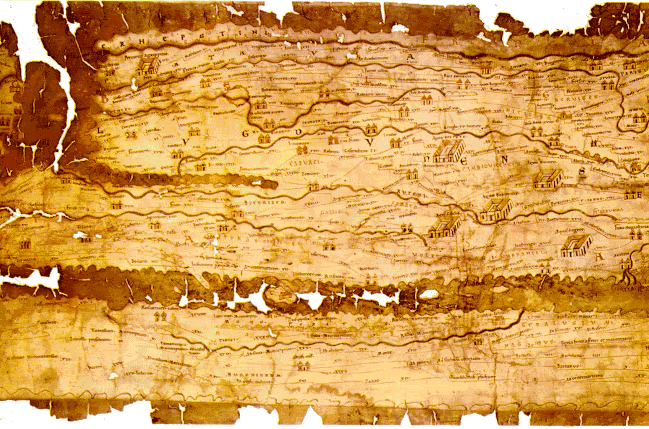
\includegraphics[width=0.4\textwidth,keepaspectratio]
        {images/history/peutinger.png}
    }
    \qquad
    \subcaptionbox
    [
      Peutinger map with Rome as central point, Urldate: 07.2016 \newline
      \small\texttt{\url{https://web.archive.org/web/20060106224928/http://www.kargi.de/Geschichte/Peutinger/peutinger_rom.jpg}}
    ]
    {
        Peutinger map with Rome as central point.
        \label{fig:peutinger-rome}
    }
    [.4\linewidth]
    {
        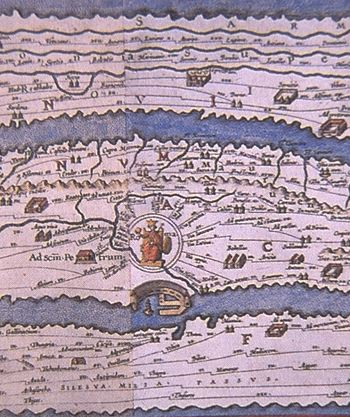
\includegraphics[width=0.4\textwidth,keepaspectratio]
        {images/history/peutinger_rom.jpg}
    }

    \caption{Varieties of the Peutinger map.}
\end{figure}


Figure \ref{fig:peutinger-rome} on page \pageref{fig:peutinger-rome} shows Rome as the central point with 12 different ways leaving it. The map was not meant to be accurate and true to scale. Its primary goal was to give travelers outline where they need to go to reach their destination. All distances on the map are graphically distorted, but the correct distances are mentioned next to the roads as numbers. Thus the map's only accuracy consists of the structure.

A Greek astronomer called Ptolemy was one of the most influential Greek astronomers and geographers of his time. He was one of the first to propound the geocentric theory of the solar system. His maps projected the earth spherical where latitude combined with longitude characterised positions. Alongside the first use of longitude in maps he also was the first one specifying terrestrial locations by celestial observations. Figure \ref{fig:ptolemy} on page \pageref{fig:ptolemy} shows a reconstructed map from Ptolemy's geography in the 15\textsuperscript{th} century, indicating ``Sinae'' at the far right, beyond the oversized island of ``Taprobane'' and the ``Aurea Chersonesus''.

\begin{figure}[!htb]
\centering
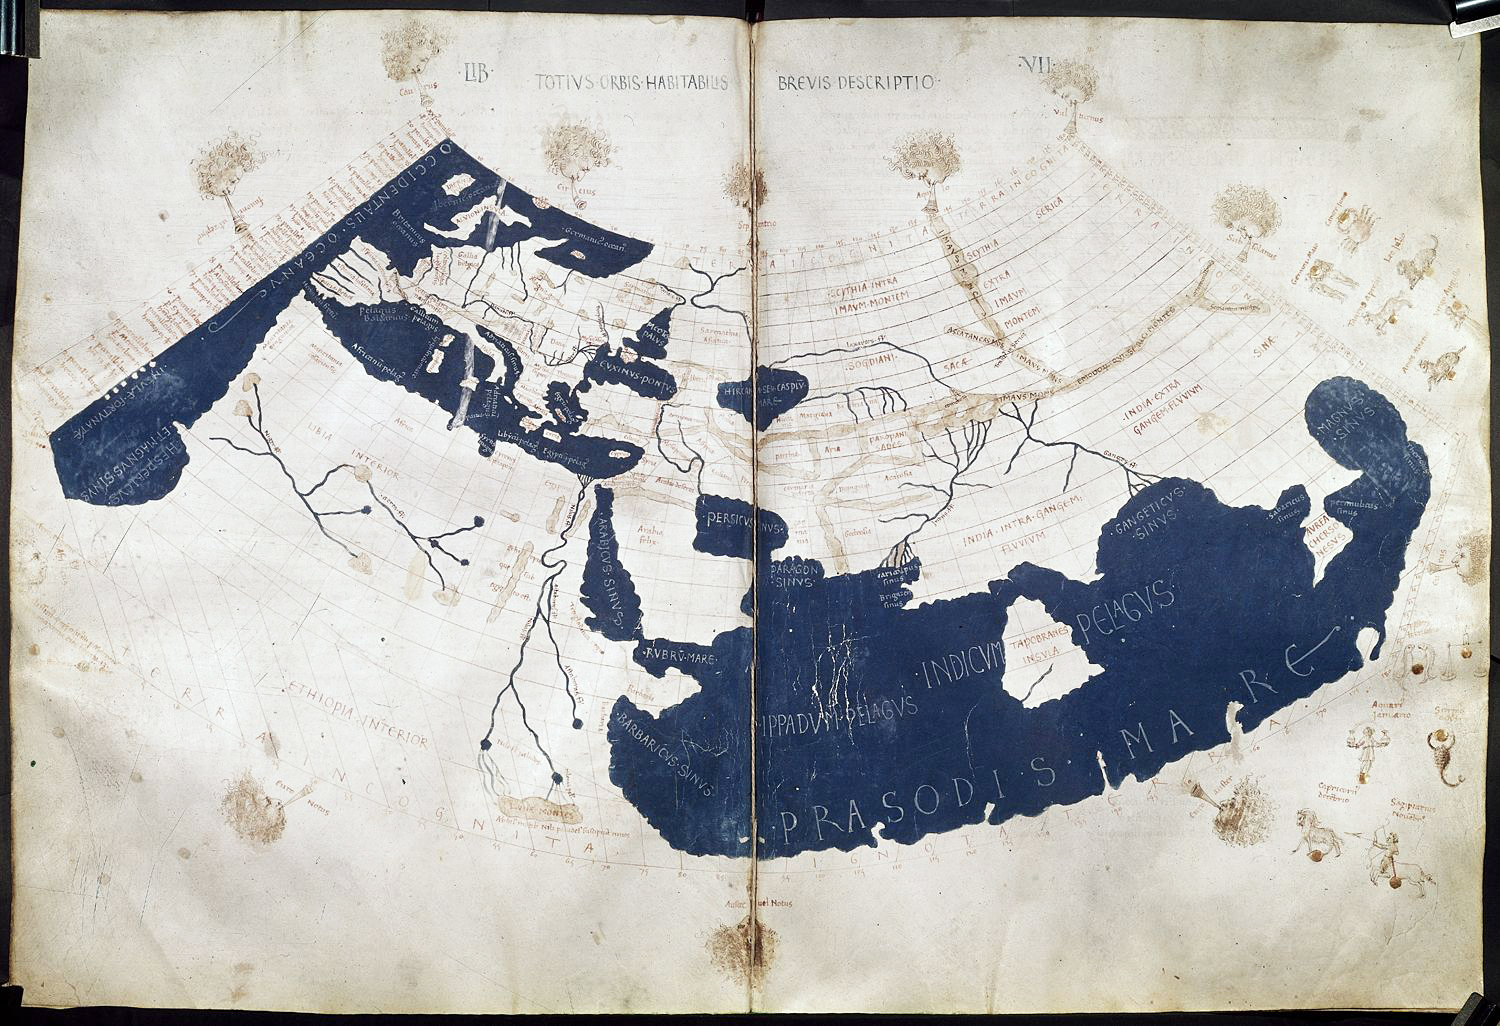
\includegraphics[width=0.8\textwidth,keepaspectratio]{images/history/ptolemy-map.jpg}
\caption[
    Reconstructed Ptolemy's map, Urldate: 07.2016 \newline
\small\texttt{\url{https://upload.wikimedia.org/wikipedia/commons/2/23/PtolemyWorldMap.jpg}}
]{Reconstructed Ptolemy's map}
\label{fig:ptolemy}
\end{figure}

% TODO: ueberleitung von maps auf andere visualisierungen
The earliest known attempt to show changing values graphically was around the 10\textsuperscript{th} century. Figure \ref{fig:planetary-movement} on page \pageref{fig:planetary-movement} tries to show planetary movement like the positions of the sun, moon, and planets throughout the year.

\begin{figure}[!htb]
\centering
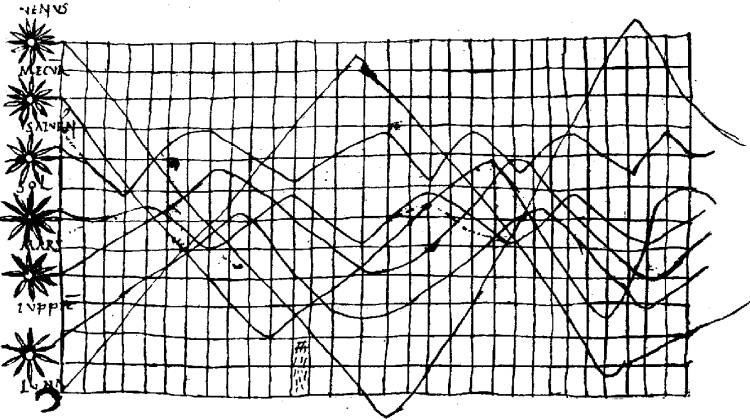
\includegraphics[width=0.4\textwidth,keepaspectratio]{images/history/planetary-movement.jpg}
\caption[
    Planetary movements, Urldate: 07.2016 \newline
\small\texttt{\url{http://www.fi.uu.nl/wiskrant/artikelen/hist_grafieken/begin/images/planeten.gif}}
]{Planetary movements}
\label{fig:planetary-movement}
\end{figure}

1350 was the year in which the first bar chart of its sort appeared and was named proto-bar graph. Oresme, a French bishop and philosopher, proposed the use of a bar graph for plotting a variable magnitude whose value depends on another. Figure \ref{fig:oresme-proto} on page \pageref{fig:oresme-proto} shows such a graph in detail and Figure \ref{fig:oresme-page} on page \pageref{fig:oresme-page} shows a page written in Latin containing different types of concepts which all implicitly have the idea of a coordinate system. The graphical use of bars also reveals the implication of the use of mathematical aggregation.

\begin{figure}[!htb]
    \centering
    \subcaptionbox
    [
      Oresme proto bar graph extracted from his concept page, Urldate: 07.2016 \newline
      \small\texttt{\url{http://datavis.ca/milestones//admin/uploads/images/icons/oresmekl.gif}}
    ]
    {
        Oresme proto bar graph extracted from his concept page.
        \label{fig:oresme-proto}
    }
  [.4\linewidth]
    {
        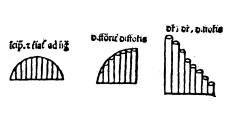
\includegraphics[width=0.4\textwidth,keepaspectratio]
        {images/history/oresme-proto.jpg}
    }
    \qquad
    \subcaptionbox
    [
      Oresmes concept page written in Latin, Urldate: 07.2016 \newline
      \small\texttt{\url{http://datavis.ca/milestones//admin/uploads/images/oresme6.gif}}
    ]
    {
        Oresmes concept page written in Latin.
        \label{fig:oresme-page}
    }
    [.4\linewidth]
    {
        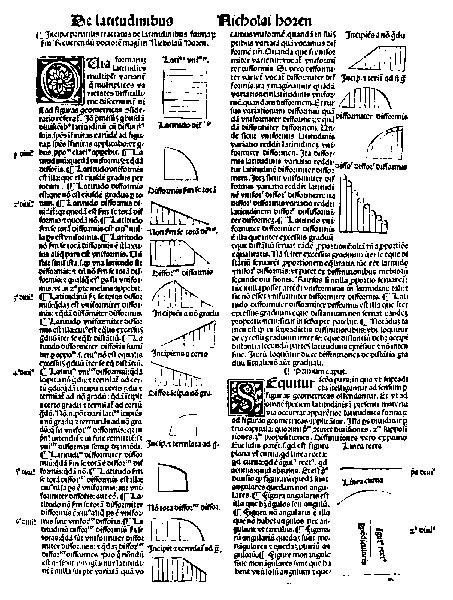
\includegraphics[width=0.4\textwidth,keepaspectratio]
        {images/history/oresme-page.jpg}
    }

    \caption{Oresmes concept page written in Latin with the extracted proto bar graphs.}
\end{figure}

25 years later, 1375, Abraham and Jehuda Cresques made the first Catalan Atlas. It consists of six images also called portolan charts which show the position of coasts and ports very accurately. All portolan charts together cover the regions from the Atlantic Ocean to China. The informations to make the atlas was gathered from sailors who used Mallorca, the hometown of Abraham and Jehuda Cresques, as a junction. Figure \ref{fig:catalan-atlas} on page \pageref{fig:catalan-atlas} shows one portolan chart displaying Europe, North Africa, and the Near East. The atlas was the first of its kind having undistorted distances between geographical regions.

\begin{figure}[!htb]
\centering
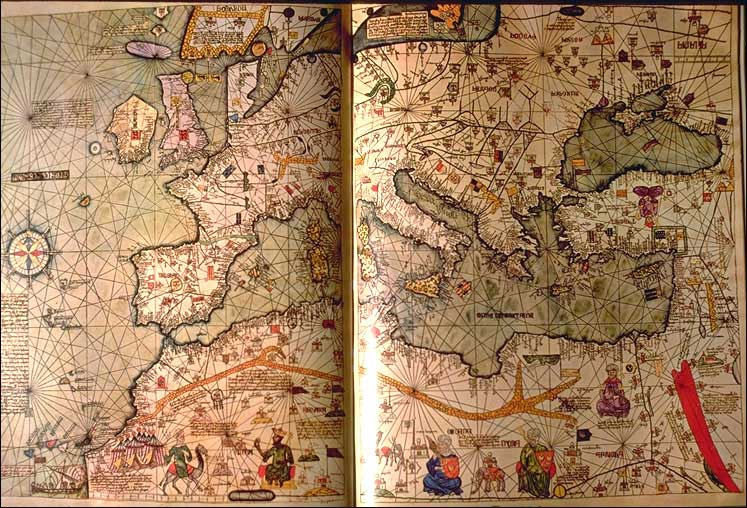
\includegraphics[width=0.8\textwidth,keepaspectratio]{images/history/catalan-atlas.jpg}
\caption[
    One out of six portolan charts of the Catalan Atlas, Urldate: 07.2016 \newline
\small\texttt{\url{http://datavis.ca/milestones//admin/uploads/images/CatalanE.jpg}}
]{One out of six portolan charts of the Catalan Atlas}
\label{fig:catalan-atlas}
\end{figure}

In 1569, Gerard Mercator invented a new map projection which bears his name. The main task for this projection was to map a world onto a cylinder in such a way that all lines of latitude have the same length as the equator. This should help sailors to lay out a course easily because a navigator needed a map where a line of constant bearing would cross all meridians at the same angle. On the one hand the projection provides very accurate directions and shapes of regions, but on the other hand, the size of regions are distorted increasingly to the north and south pole. Figure \ref{fig:mercator} on page \pageref{fig:mercator} shows a map of the world with a Mercator projection.

\begin{figure}[!htb]
\centering
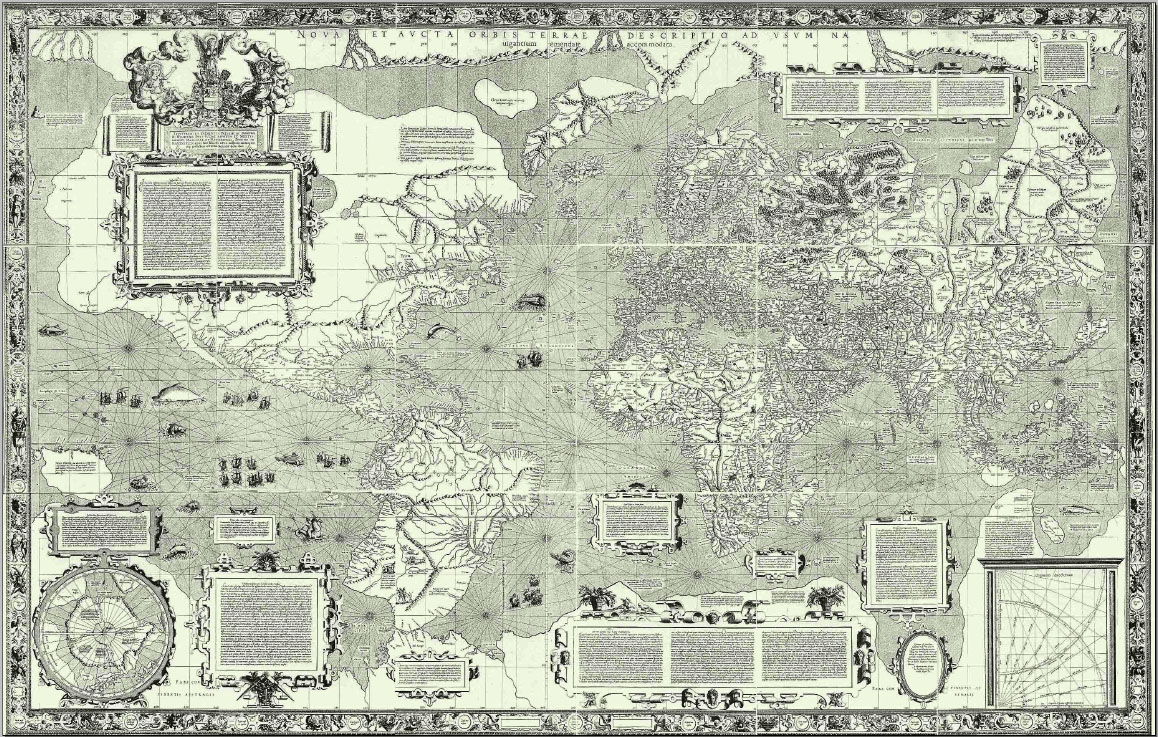
\includegraphics[width=0.8\textwidth,keepaspectratio]{images/history/mercator.png}
\caption[
    A map of the world with a Mercator projection, Urldate: 07.2016 \newline
\small\texttt{\url{https://upload.wikimedia.org/wikipedia/commons/b/b2/Mercator_1569.png}}
]{A map of the world with a Mercator projection}
\label{fig:mercator}
\end{figure}

One year later, 1570, the first modern atlas named Theatrum Orbis Terrarum (``Theatre of the World''), or Ortelius-Atlas appeared. It was a book consisting of a collection of uniform map sheets and sustaining text bounds. The collection of map sheets included not a single map made by Ortelius. At first, it bundled maps from 53 other cartographers with the source. However, Ortelius brought consistency to all those maps. He dropped the maps all in the same style and size and arranged them logically by continent, region, and state. Nevertheless, the naming and location coordinates were not normalised. Figure \ref{fig:ortelius} on page \pageref{fig:ortelius} shows a world map in Theatrum Orbis Terrarum. Ortelius also regularly revised and expanded the atlas making it the first economically successful one.

\begin{figure}[!htb]
\centering
\includegraphics[width=0.8\textwidth,keepaspectratio]{images/history/ortelius.jpeg}
\caption[
    A map of the world in the Ortelius atlas, Urldate: 07.2016 \newline
\small\texttt{\url{https://upload.wikimedia.org/wikipedia/commons/6/6f/OrteliusWorldMap.jpeg}}
]{A map of the world in the Ortelius atlas}
\label{fig:ortelius}
\end{figure}

1626 the idea of \textit{small multiples} got proposed. It was used to show a series of images in a coherent display. The origin of the idea is based in displaying the changes in sunspots over time in a visual representation as Figure \ref{fig:small-multiples} on page \pageref{fig:small-multiples} shows.

\begin{figure}[!htb]
\centering
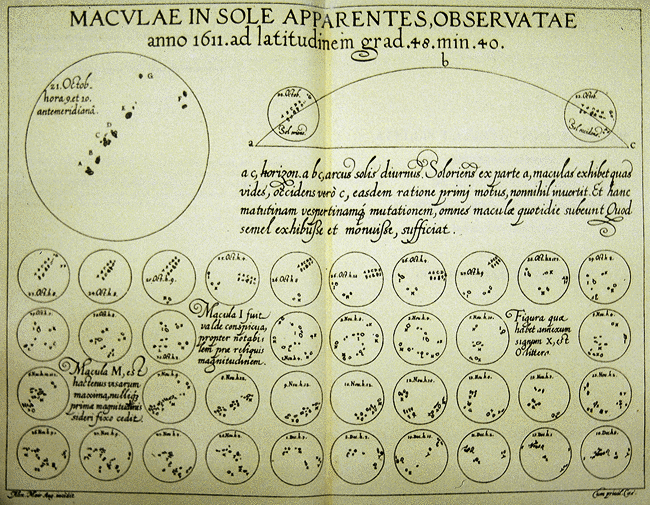
\includegraphics[height=5cm,keepaspectratio]{images/history/small-multiples.png}
\caption[
    Sunspot plate from Scheiner's ``Tres Epistolae'' using small multiples, Urldate: 07.2016 \newline
\small\texttt{\url{http://cnx.rice.edu/content/m11970/latest/tres_epistolae.gif}}
]{Sunspot plate from Scheiner's ``Tres Epistola'' using small multiples}
\label{fig:small-multiples}
\end{figure}

20 years later the first visual representation of statistical data was made. Langren showed the variations in determination of longitude between Toledo and Rome (see Figure \ref{fig:langren} on page \pageref{fig:langren}). The left-most location is the starting point in this visualisation. The distance to other locations is shown as a number line.

\begin{figure}[!htb]
\centering
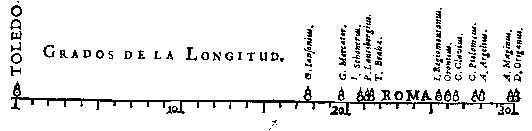
\includegraphics[width=0.8\textwidth,keepaspectratio]{images/history/langren.jpg}
\caption[
    First data graph showing variations in determination of longitude between Toledo and Rome, Urldate: 07.2016 \newline
\small\texttt{\url{http://datavis.ca/milestones//admin/uploads/images/tufte/langren.jpg}}
]{First data graph showing distance between different locations.}
\label{fig:langren}
\end{figure}

In the 18\textsuperscript{th} century, cartographers began to try to show more than one channel on a map (the term \textit{channel} is explained in detail in Chapter \ref{s:basics} on page \pageref{s:basics}). Up to now the only channel used on a map was the a geographical position only. As a result, new graphic forms such as contours lines, or also called isolines, got invented, and thematic mapping of physical quantities took root. Towards the end of this century, the first attempts at thematic mapping of geologic, economic, and medical data are available.

The first half of the 19\textsuperscript{th} century witnessed a tremendous growth in statistical graphics and thematic mapping because of the fertilization provided by previous innovations of design and technique. All modern forms of data visualisations now known as bar and pie charts, histograms, line graphs and time-series plots, contour plots and so forth, have been invented. In the field of cartography, a shift from single geographical maps to comprehensive atlases, depicting data on a wide variety of topics (economic, social, medical, physical, etc.) happened. As an example, Figure \ref{fig:first-choropleth} on page \pageref{fig:first-choropleth} features the first choropleth map (for more information about choropleth maps see Chapter \ref{s:choropleth} on page \pageref{s:choropleth}). It shows the distribution and intensity of illiteracy in France.

\begin{figure}[!htb]
    \centering
    \subcaptionbox
    [
      First choropleth map showing the distribution and intensity of illiteracy in France, Urldate: 07.2016 \newline
      \small\texttt{\url{http://datavis.ca/milestones//admin/uploads/images/dupin.gif}}
    ]
    {
        First choropleth map showing the distribution and intensity of illiteracy in France.
        \label{fig:first-choropleth}
    }
  [.4\linewidth]
    {
        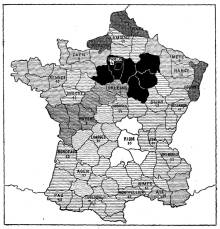
\includegraphics[width=0.4\textwidth,keepaspectratio]
        {images/history/dupin.jpg}
    }
    \qquad
    \subcaptionbox
    [
      The first comparative choropleth thematic maps, showing crimes against persons and crimes against property in relation to level of instruction by departments in France, Urldate: 07.2016 \newline
      \small\texttt{\url{http://datavis.ca/milestones//admin/uploads/images/guerry/guerry-balbi-600s.jpg}}
    ]
    {
        The first comparative choropleth thematic maps, showing crimes against persons and crimes against property in relation to level of instruction by departments in France.
        \label{fig:second-choropleth}
    }
    [.4\linewidth]
    {
        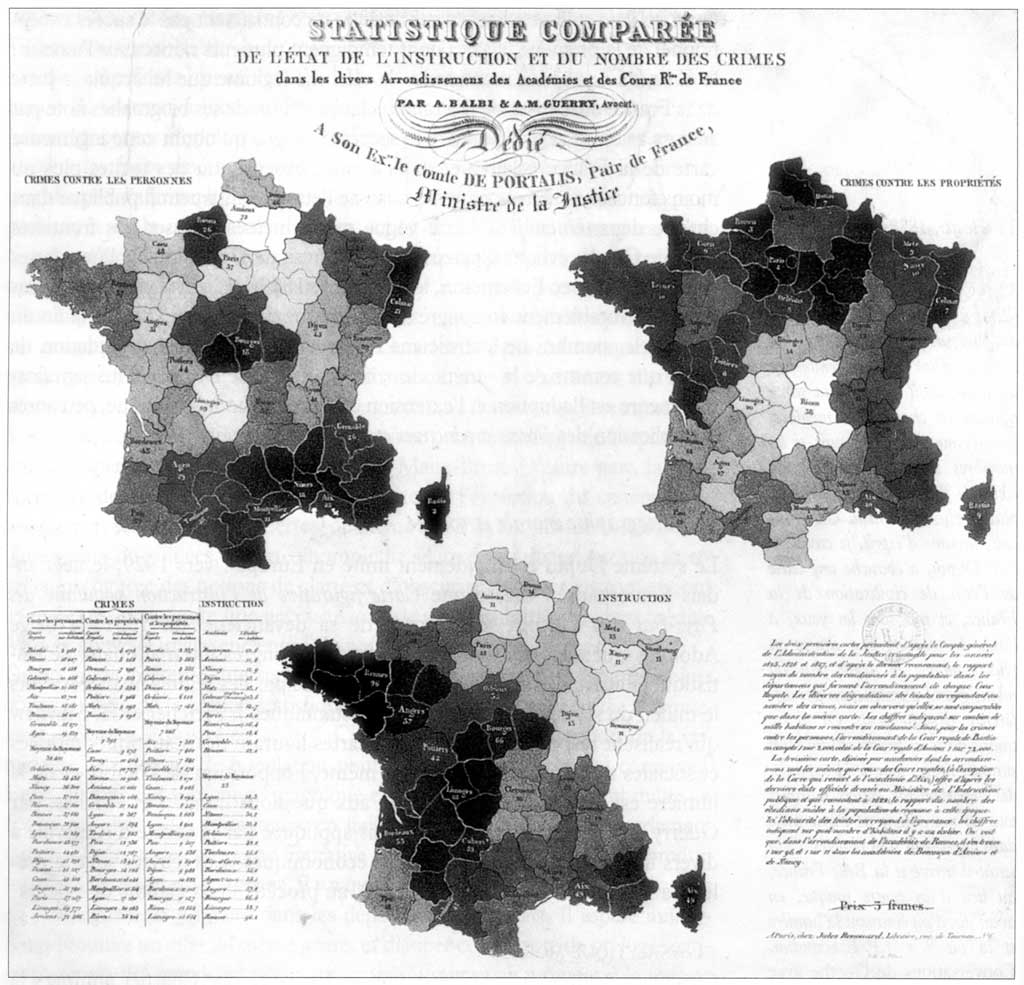
\includegraphics[width=0.4\textwidth,keepaspectratio]
        {images/history/second-choropleth.jpg}
    }
    \caption{The first variations of choropleth maps.}
\end{figure}

This map was followed shortly by comparative choropleth thematic maps, showing crimes against persons and crimes against property in relation to the level of instruction by departments in France (see Figure \ref{fig:second-choropleth} on page \pageref{fig:second-choropleth}.).

1830 the first dot map of population appeared in France. Each dot represents 10.000 people in the department (see Figure \ref{fig:first-dotmap} on page \pageref{fig:first-dotmap}.).

\begin{figure}[!htb]
\centering
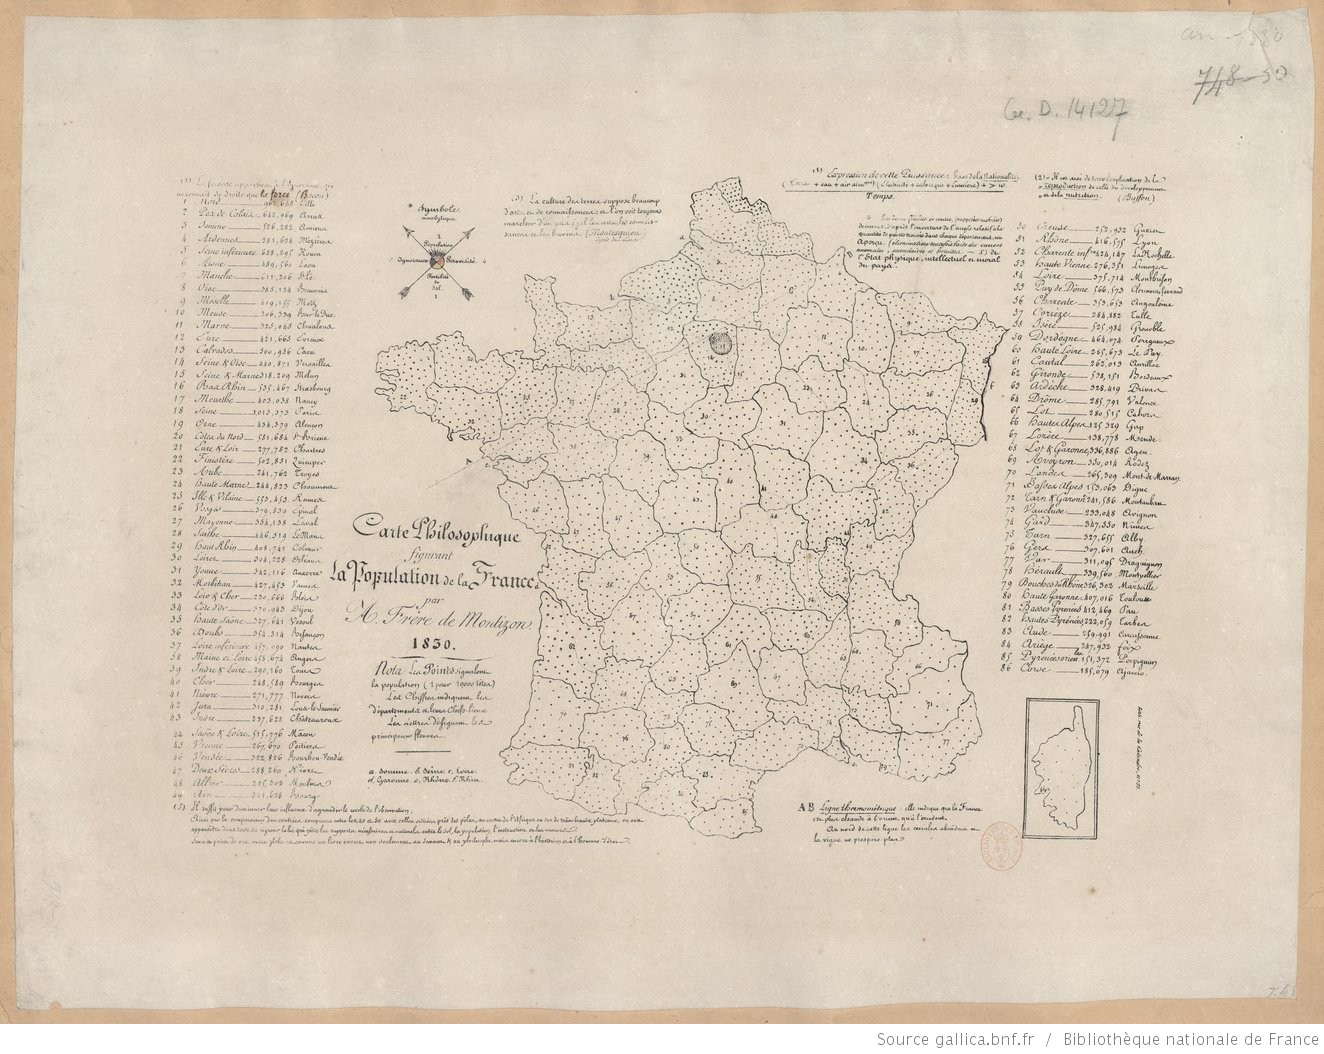
\includegraphics[width=0.8\textwidth,keepaspectratio]{images/history/montizon-dotmap2.jpeg}
\caption[
    The first dot map of population by department, 1 dot = 10.000 people, Urldate: 07.2016 \newline
\small\texttt{\url{http://gallica.bnf.fr/ark:/12148/btv1b8492261j/f1.highres}}
]{The first dot map of population by department, 1 dot = 10.000 people}
\label{fig:first-dotmap}
\end{figure}

The second half of the 19\textsuperscript{th} century is also known as ``the golden age of data graphics''. All the conditions for tremendous growth of visualisations were given once again: throughout Europe official state statistical offices were established.
Statistical theory (initiated by Gauss and Laplace) provided the means to make sense of large bodies of data.
This half of the century included the first mixture of a map with a diagram: Figure \ref{fig:first-mixture} on page \pageref{fig:first-mixture} shows a map using pie charts to represent the cattle sent from all around France for consumption in Paris.

\begin{figure}[!htb]
\centering
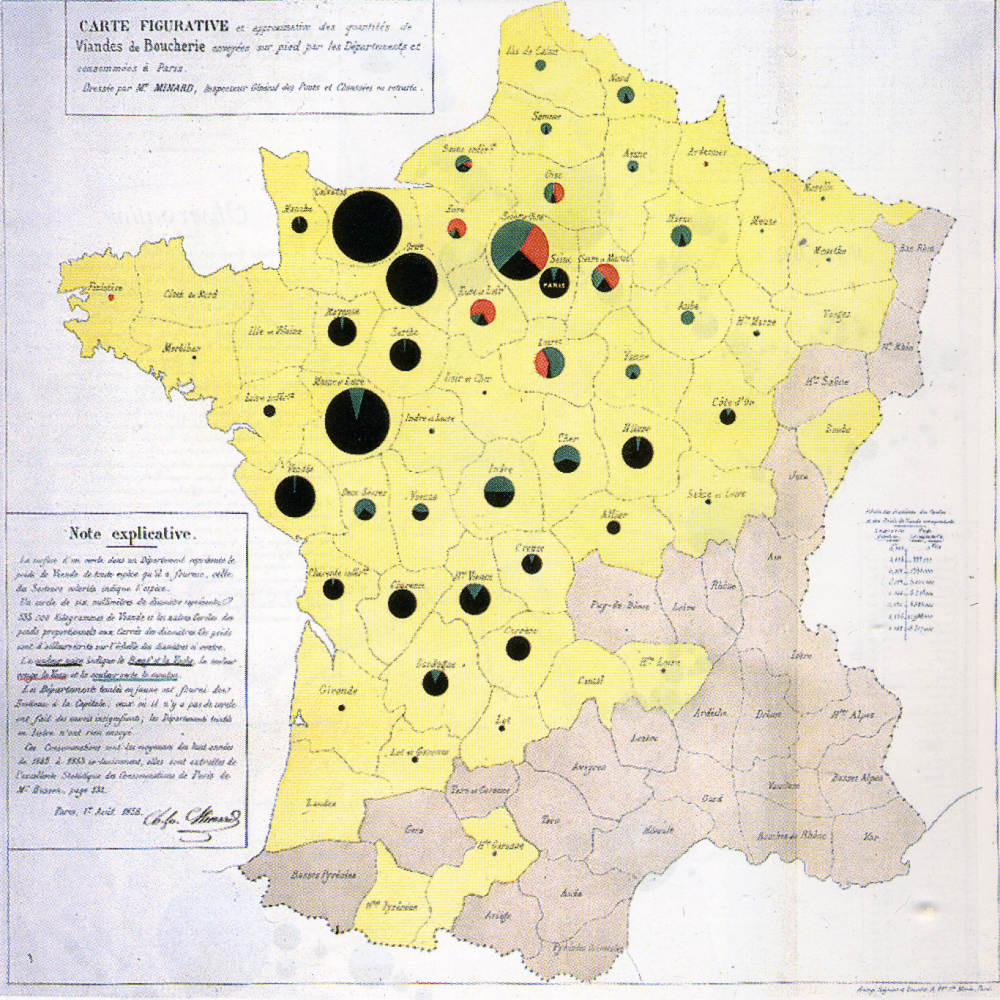
\includegraphics[width=0.4\textwidth,keepaspectratio]{images/history/minard.png}
\caption[
    A map using pie charts to represent the cattle sent from all around France for consumption in Paris., Urldate: 07.2016 \newline
\small\texttt{\url{https://upload.wikimedia.org/wikipedia/commons/1/1c/Minard-carte-viande-1858.png}}
]{A map using pie charts to represent the cattle sent from all around France for consumption in Paris.}
\label{fig:first-mixture}
\end{figure}

Another well-known example of graphical representation from that century is the so-called ``cholera map'' (see Figure \ref{fig:cholera-map} on page \pageref{fig:cholera-map}.). Here, a dot map is used to display epidemiological data. This map could be used for knowledge creation in terms of the discovery of the source of a cholera epidemic. It showed that a high number of deaths were occurring near a water pump.

\begin{figure}[!htb]
\centering
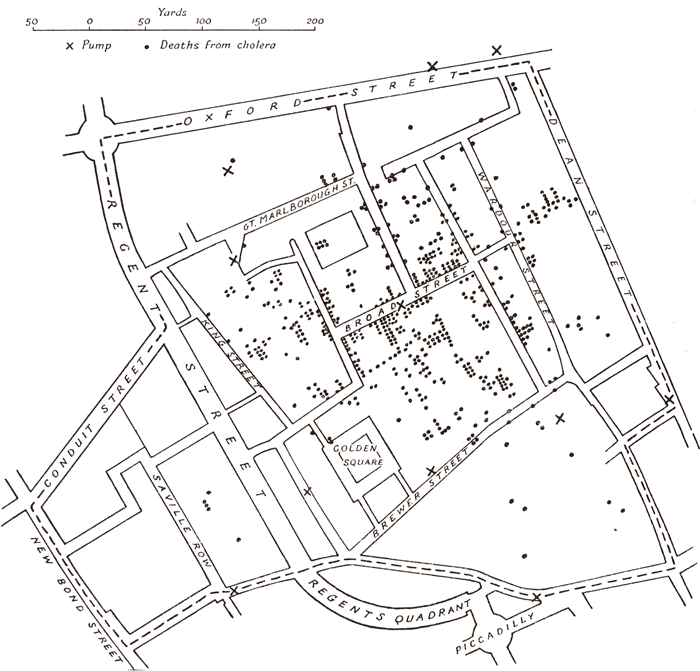
\includegraphics[width=0.8\textwidth,keepaspectratio]{images/history/cholera2.png}
\caption[
    Dot map showing the clusters of cholera cases in the London epidemic of 1854., Urldate: 07.2016 \newline
\small\texttt{\url{http://datavis.ca/milestones//admin/uploads/images/tufte/snow.gif}}
]{Dot map showing the clusters of cholera cases in the London epidemic of 1854.}
\label{fig:cholera-map}
\end{figure}

In 1861, a new channel appeared in map-based visualisations. It represents a weather map with glyphs where each glyph embodies air pressure and barometric changes by means. Figure \ref{fig:weather-map} on page \pageref{fig:weather-map} shows the mentioned weather map.

\begin{figure}[!htb]
\centering
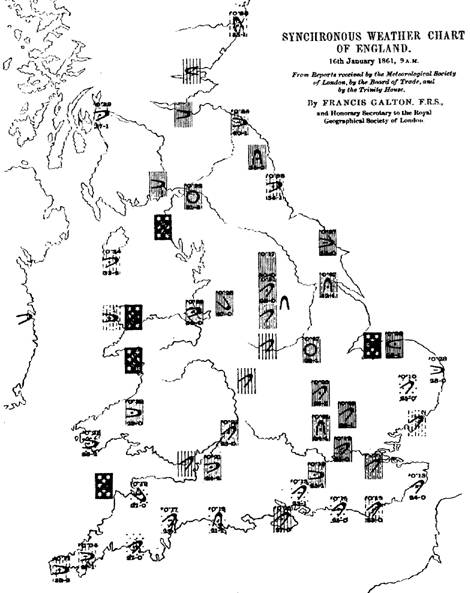
\includegraphics[width=0.4\textwidth,keepaspectratio]{images/history/weather.jpg}
\caption[
    A chart showing area of similar air pressure and barometric changes by means of glyphs displayed on a map., Urldate: 07.2016 \newline
\small\texttt{\url{http://datavis.ca/milestones//admin/uploads/images/galton-weather-charts2.gif}}
]{A chart showing area of similar air pressure and barometric changes by means of glyphs displayed on a map.}
\label{fig:weather-map}
\end{figure}

Eight years later, Napoleon's march on Moscow (also called ``the best graph ever produced'') was visualised by Minard and is shown in Figure \ref{fig:minard2} on page \pageref{fig:minard2}. Overall this figurative map can be described as the ``Map of the successive losses in men of the French Army in the Russian campaign 1812-1813''. The reason why this graph is sometimes referred to as the best graph ever produced is that it contains multiple visual channels without influencing the comprehensibility of the graph. The following list describes some of the values encoded in the graph:
\begin{itemize}
\item The number of men alive is encoded by the thickness of the colored lines at a rate of one millimeter for 10.000 men. The exact amount of men alive is also written beside the zones.
\item The color of the lines indicates the moving direction of the troops. Brown designates men moving into Russia and black are those on retreat.
\item The temperature is plotted at different points along the retreat at the bottom.
\end{itemize}
All in all, Figure \ref{fig:minard2} on page \pageref{fig:minard2} encodes six different types of data in two dimensions:
\begin{enumerate*}[label={(\arabic*)}]
\item the number of Napoleon's troops,
\item the distance traveled
\item temperature
\item latitude and longitude
\item direction of travel and
\item location relative to specific dates.
\end{enumerate*}
As of today, such a visual representation is known as a Sankey diagram which is a specific type of a flow diagram.

\begin{figure}[!htb]
\centering
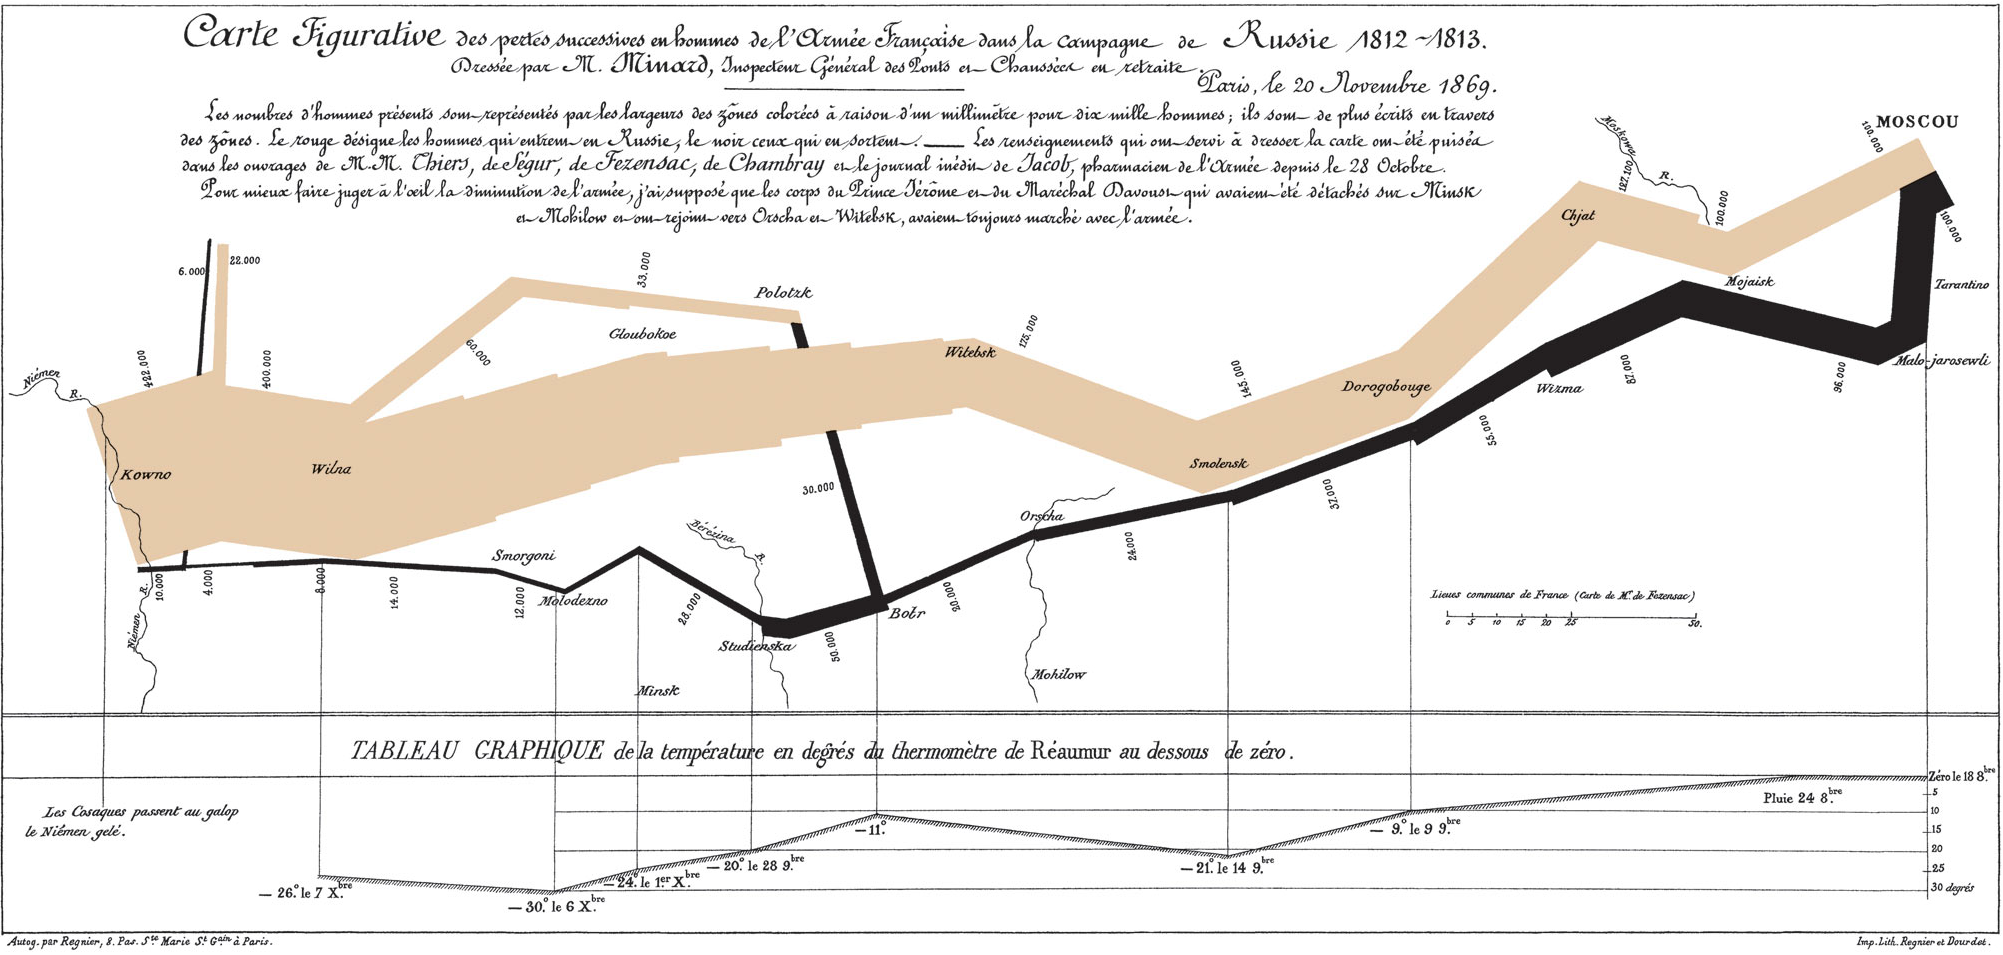
\includegraphics[width=0.8\textwidth,keepaspectratio]{images/history/minard2.png}
\caption[
    Charles Minard's map of Napoleon's disastrous Russian campaign of 1812., Urldate: 07.2016 \newline
\small\texttt{\url{https://upload.wikimedia.org/wikipedia/commons/2/29/Minard.png}}
]{Charles Minard's map of Napoleon's disastrous Russian campaign of 1812.}
\label{fig:minard2}
\end{figure}

If the literature refers to the 19\textsuperscript{th} century as ``the golden age'', they also often refer to the first half of the 20\textsuperscript{th} century as the ``modern dark ages'' of visualisation. Only a few graphical innovations arisen because in this period statistical graphics became to be standard practice. Nonetheless, visual representations were used to provide new insights, discoveries, and theories in this period. This was probably the first time graphical methods were used in different research fields such as astronomy, physics, and other sciences to justify hypotheses. Another research, which had much impact in the research field of visualisation, was about comparisons of the efficacy of various graphic forms. In the mid-1960s, three developments made a significant impact on data visualisations:
\begin{enumerate}
\item \ac{EDA} was first mentioned by John W. Tukey in a paper called ``The Future of Data Analysis''. He demanded a strict distinction between data analysis as a legitimate branch of statistics and mathematical statistics.
\item The book called ``Sémiologie graphique'' (Semiology of graphics) was written and published by Jacques Bertin. To some
\begin{quote}
``[\ldots] this appeared to do for graphics what Mendeleev had done for the organization of the chemical elements, that is, to organize the visual and perceptual elements of graphics according to the features and relations in data \iacite{Friendly.2001}.''
\end{quote}
\label{crossref:bertain}
\item Computer processing of data arisen, which offered more flexibility and possibilities in constructing graphic forms by programs.
\end{enumerate}

By the end of the 20\textsuperscript{th} century, new research fields emerged and significant intersections and collaborations began: computer science research combined with the developments in data analysis provided new paradigms, languages, and helpful packages to create statistical and data graphics. Thus a tremendous growth in new visualisation methods and techniques appeared anew.
Another important innovation in that period were new paradigms  concerning direct manipulation of data (linking, brushing, selection, focus, etc. (for a detailed explanation see Chapter \ref{s:basics} on page \pageref{s:basics}.)).